%Compile with PDFLaTeX
\documentclass[a4paper,10pt,english]{article}
\usepackage{mathptmx}
\renewcommand{\familydefault}{\rmdefault}
\usepackage{graphicx}
\usepackage{babel}
\usepackage{caption}
\usepackage{subcaption}
\usepackage{floatrow}
\usepackage{orstylet}
\makeatother
\begin{document}
\renewcommand{\figurename}{Fig.} 


\title{Estimating the fake lepton backgrounds for the Drell-Yan differential cross section measurement using 2016 CERN CMS data}


\author{\uline{Marijus Ambrozas}, Andrius Juodagalvis}

\maketitle

\address{Institute of Theoretical Physics and Astronomy, Faculty of Physics, Vilnius University, Lithuania}

\rightaddress{marijus.ambrozas@ff.stud.vu.lt}

The Drell-Yan process takes place during a proton-proton collision when a quark and an antiquark annihilate to create an
oppositely charged lepton pair through an s-channel exchange of a $Z$ boson or a virtual photon
($q\bar{q}\rightarrow Z/\gamma^*\rightarrow l^+l^-$) \cite{DY}.
Precise measurements of the Drell-Yan differential cross section are used to constrain the parton distribution functions
which describe the inner structure of the proton as well as to test the perturbative framework of the standard model \cite{DY13}.
These measurements are also important for a number of other experimental analyses where the Drell-Yan process is considered a
background \cite{Higgs, Zprime, SUSY}.

At the Large Hadron Collider where the protons get smashed with 13~TeV center-of-mass energy, the resulting leptons from the Drell-Yan
process usually have high momenta and are well separated from tracks of other particles.
Such leptons are often called ``prompt.''
Other processes exist which can produce the same final state as the Drell-Yan process.
They are referred to as prompt lepton backgrounds.
However, there are also some non-prompt or so-called ``fake'' lepton backgrounds.
These backgrounds appear when a poorly isolated lepton emerging from a hadronic jet or even the jet itself
gets misreconstructed as a prompt lepton.
The most probable fake lepton backgrounds are the $W$+Jets ($W$ boson produces a prompt lepton and the jet produces a fake one)
and the $QC\!D$ multijet (all leptons in the event are fake) processes.

Fake lepton processes are very difficult to simulate as they have very large cross sections and very low probabilities to be
considered as Drell-Yan event candidates.
Therefore, such backgrounds are estimated using a data-driven approach.
Two potentialy appropriate methods were explored and will be presented and compared during the presentation:
\begin{enumerate}
\item The ``fake rate'' method relies on measuring the fake lepton selection efficiency. It is then
applied on events containing fake leptons that have failed the event selection to estimate the number of
events that have passed it.
\item The ``matrix'' method is a more sophisticated method as it additionally relies on
the prompt lepton selection efficiency.
\end{enumerate}

The analysis was made using 2016 CERN CMS data recorded at $\sqrt{s}=13$ TeV in collaboration with scientists
from Universit\'{e} libre de Bruxelles, Yonsei University, and the University of Nebraska in Lincoln.
 
\vspace{-0.3cm}
\begin{figure}[H]
	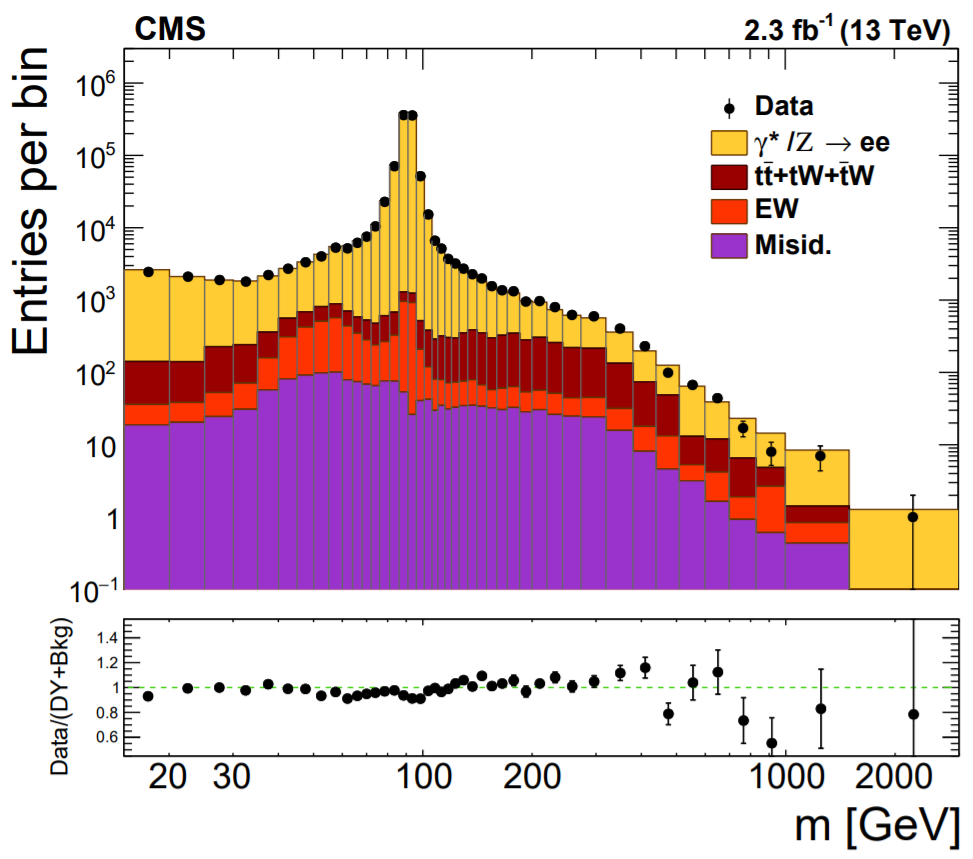
\includegraphics[width=.45\linewidth]{Figure1.png}
	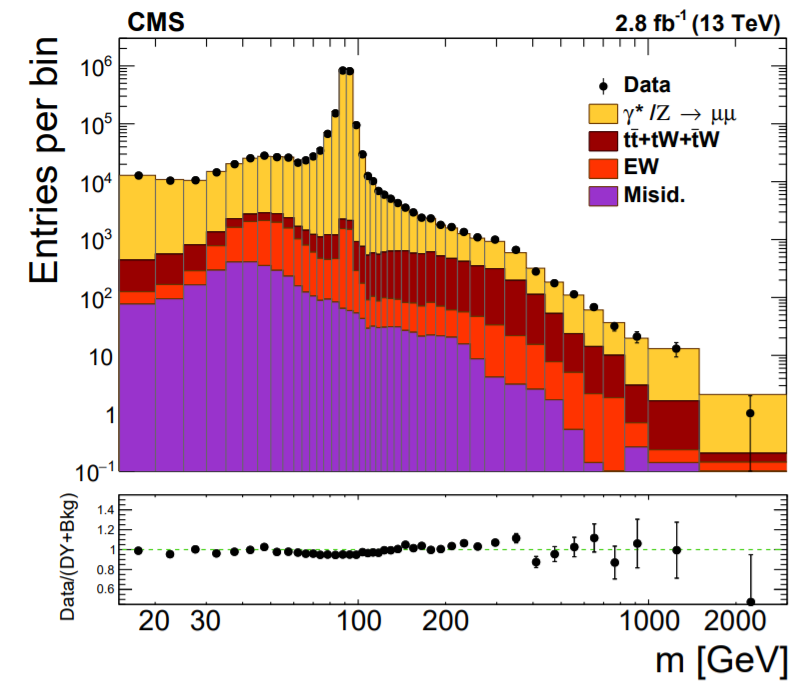
\includegraphics[width=.45\linewidth]{Figure2.png}
\vspace{-0.2cm}
\caption{Dielectron and dimuon (left and right plot) invariant mass spectra measured using 2015 CERN CMS data \cite{DY13}.
      Black dots show event counts measured with the CMS detector.    
      Yellow bars denote simulated DY signal.
      The ``EW'' label indicates the contributions from the DY production of $\tau^+\tau^-$, $WW$, $WZ$, and $ZZ$ processes.
      The ``Misid.'' label corresponds to $W$+Jets and $QC\!D$ multijet backgrounds.}
\end{figure}

\vspace{-0.5cm}
\begin{thebibliography}{References}
\bibitem{DY}S.\ D.\ Drell, T.\ M.\ Yan, Massive Lepton Pair Production in Hadron-Hadron Collisions at High-Energies,
Phys.\ Rev.\ Lett.\ \textbf{25}, 316 (1970).

\bibitem{DY13}CMS Collaboration, Measurement of the differential Drell-Yan cross section in proton-proton collisions
at $\sqrt{s}=13$ TeV, JHEP \textbf{12} 059 (2019).

\bibitem{Higgs}ATLAS Collaboration. A search for the dimuon decay of the Standard Model Higgs boson with the ATLAS detector.
Phys.\ Lett.\ B \textbf{812}, 135980 (2021).

\bibitem{Zprime}CMS Collaboration. Search for high-mass resonances in dilepton final states in proton-proton collisions
at $\sqrt{s}=13$ TeV. JHEP \textbf{06} 120 (2018).

\bibitem{SUSY}CMS Collaboration. Search for top squark pair production using dilepton final states in pp collision data
collected at $\sqrt{s}=13$ TeV. Eur.\ Phys.\ J.\ C \textbf{81} 3 (2021).
\end{thebibliography}

\end{document}
